\chapter{Introduction and research statement}
A \textit{software process} is a set of activities performed in order to design, develop and maintain software systems. Examples of such activities are design methods: requirements collection and creation of UML diagrams; or testing strategies: requirements testing or performance analysis. The intent behind the software process is to structure and coordinate human activities in order to achieve the goal - deliver a software system.

Many work has been done in the software process research field aiming better understanding of the software process. This work resulted in a number of industrial standards for process models: CMM, ISO, PSP etc. \cite{citeulike:5043104} which are widely accepted by many institutions. Nevertheless, the software development process stays error-prone and more than a half of all software development projects ending up failing or very poorly executed for many reasons. Some of them getting abandoned while running out of budget, some delivered with so low quality or so late that they become useless, and some, when delivered, never get used because they do not fulfill original requirements. The cost of this lost effort is enormous and this facts clearly reveal our incomplete knowledge of the software process.

There is a long history of software process improvement through proposing specific patterns of software development process. For example, the Waterfall Model process proposes a sequential pattern in which developers first create a Requirements document, then create a Design, then create an Implementation, and finally develop Tests. The Test Driven Development process proposes an iterative pattern in which the developer must first write a test case, then write the code to implement that test case, then refactor the system for maximum clarity and minimal code duplication. One problem with the traditional top-down approach to process development is that it requires the developer or manager to notice a recurrent pattern of behavior in the first place \cite{citeulike:5043104}. 

In my research, I will apply knowledge discovery and data mining techniques to the domain of software engineering in order to evaluate their ability to automatically notice interesting recurrent patterns of behavior. While I am not envisioning to be able to infer a full complete and correct software process models, my system will provide a user with some formal description of discovered recurrent behaviors in the software process. As a simple example, consider a development team in which committing code to a repository triggers a build of the system. Sometimes the build passes, and sometimes the build fails. To improve the productivity of the team, it would be useful to be aware of any recurrent behaviors of the developers. My system might generate one recurrent pattern consisting of a) implementing code b) running unit tests, c) committing code and d) a passed build: $i \rightarrow u \rightarrow c \rightarrow s $, and another recurrent pattern consisting of a) implementing code, b) committing code, and c) a failed build: $i \rightarrow c \rightarrow f $. The automated generation of these recurrent patterns can provide actionable knowledge to developers; in this case, the insight that running test cases prior to committing code reduces the frequency of build failures.

Although, latest trends in the software process study emphasize mining of the software process artifacts and behaviors \cite{citeulike:5043664} \cite{citeulike:1885717} \cite{citeulike:5112229} \cite{citeulike:1885717}, to the best of my knowledge, the approach I am taking through the mining of automatically collected, low-level product and process data has never been attempted mainly due to the lack of the means of automated real-time data collection. By leveraging Hackystat ability of collecting such a fine grain data I am going to extend the previous research with new knowledge aiming improvements in our knowledge of the software process.

\section{Proposed contribution}
In summary, the proposed contributions of my research will include: 
\begin{itemize}
	\item the implementation of a system aiding in discovery of novel software process knowledge through the indexing of the low-level software process telemetry streams;
	\item my experimental evaluation of the system, which will provide insight into its strengths and weaknesses;
	\item the possible discovery of useful new software process patterns.
\end{itemize}


\begin{figure}[tbp]
   \centering
   \includegraphics[height=65mm]{system_overview.eps}
   \caption{The high-level system overview. Software engineering process and product data collected and aggregated by Hackystat used to generate temporal symbolic indexes. Data mining tools constrained by the software engineering domain knowledge are then used for unsupervised patterns discovery. The GUI provides an expert interface for discovered patterns and knowledge base aiding iterative investigation of a discovered phenomena.}
   \label{fig:system_overview}
\end{figure}

\section{Roadmap}
The proposal has the following organization:
\begin{itemize}
	\item Chapter \ref{related.work} presents a review of the literature in the general process discovery with application to the software process up to date. The methods discussed in this chapter are the high-level frameworks which are used for the process inference from the abstracted process artifacts.
	\item Chapter \ref{methods} presents a literature review of the temporal pattern discovery methods which I am using for the construction of the symbolic time-point, interval and event streams.
	\item Chapter \ref{trajectory} describes the requirements and presents the current state of Software Trajectory framework for automated software process discovery.
	\item Chapter \ref{experiments} describes a pilot study results and outlines planned experimental evaluation of my research.
	\item Chapter \ref{contribution} discusses anticipated contribution in greater details.
	\item Appendix (\ref{appendix}) presents the estimated timeline.
\end{itemize}
